\section{ Role of Gates: Motivation }
In this paper, we take the `path-view': the output of a DNN is obtained as a summation of the contribution of individual paths, which is possible due to the gating property of the ReLU activations. Each path contains gates and weights, and the contribution of a path is the product of the gates and the weights in the path. We now discuss the role of gates in a DNN, by splitting them into i) \emph{active} gates which are `on' gates, and ii) \emph{sensitive} gates which are near $0$ and can flip from $0$ to $1$ or vice-versa based on gradient information.
\FloatBarrier
\begin{figure}[h]
\centering
%\begin{minipage}{0.75\columnwidth}
\resizebox{\columnwidth}{!}{
\begin{tabular}{ccc}
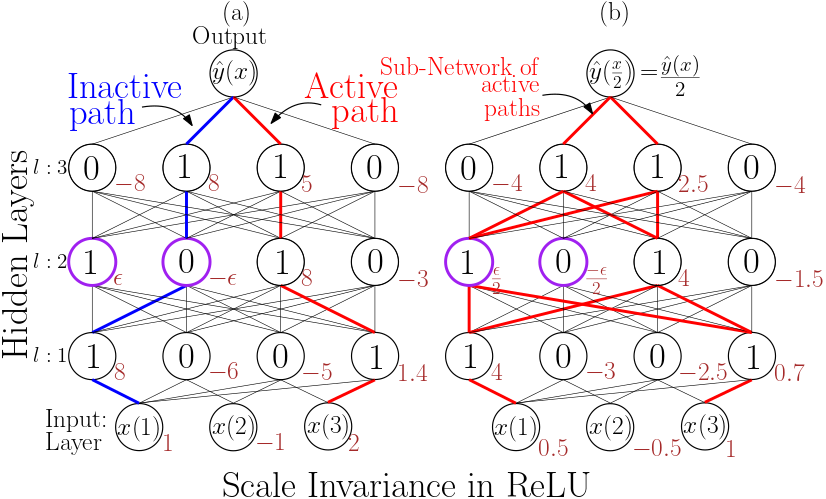
\includegraphics[scale=0.5]{figs/nn-subnet.png}
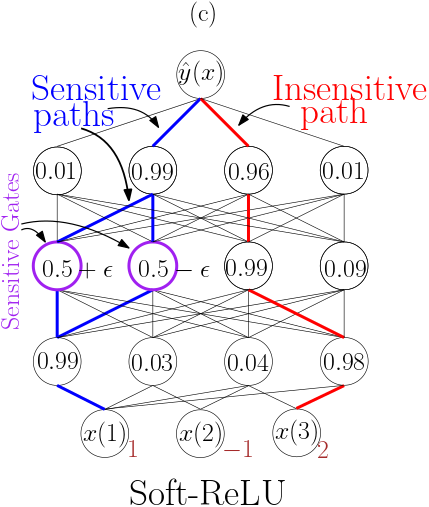
\includegraphics[scale=0.5]{figs/nnsoft.png}
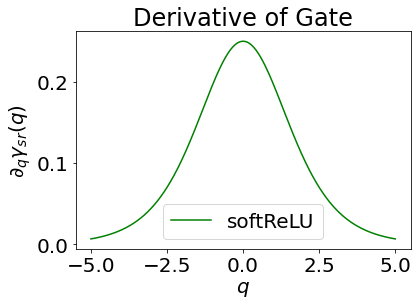
\includegraphics[scale=0.6]{figs/der-gate.png}
%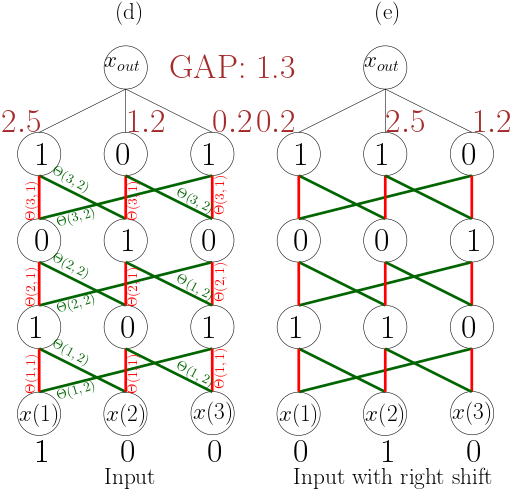
\includegraphics[scale=0.5]{figs/nnconv-size2.png}
%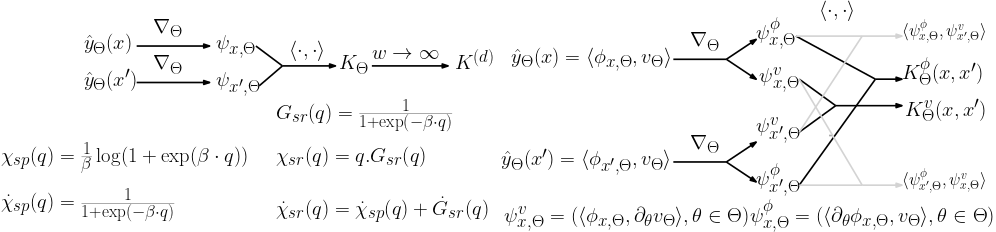
\includegraphics[scale=0.5]{figs/gradflow.png}
%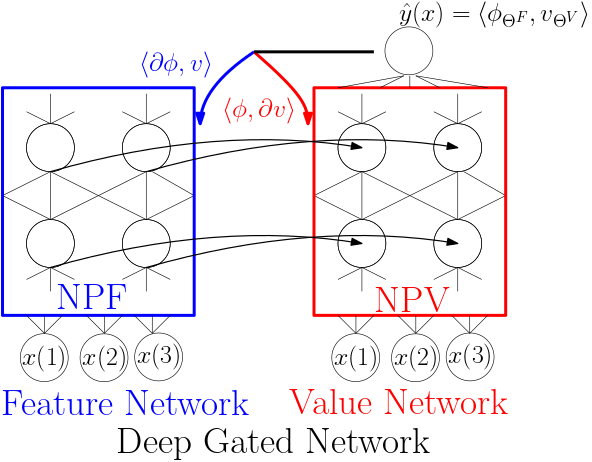
\includegraphics[scale=0.5]{figs/nntwin-blck.png}
%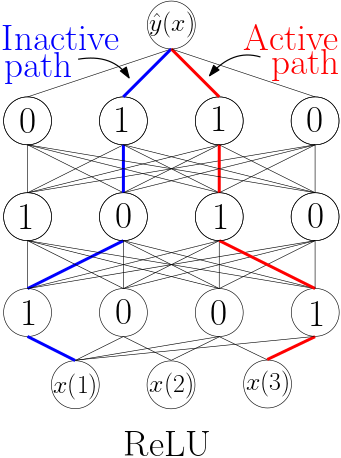
\includegraphics[scale=0.5]{figs/nn.png}
%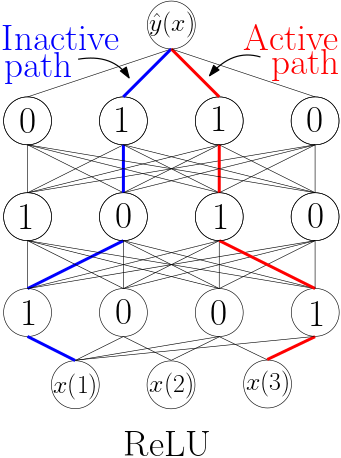
\includegraphics[scale=0.5]{figs/nn.png}
\end{tabular}
}
%\end{minipage}
%\begin{minipage}{0.18\columnwidth}
%\resizebox{\columnwidth}{!}{
%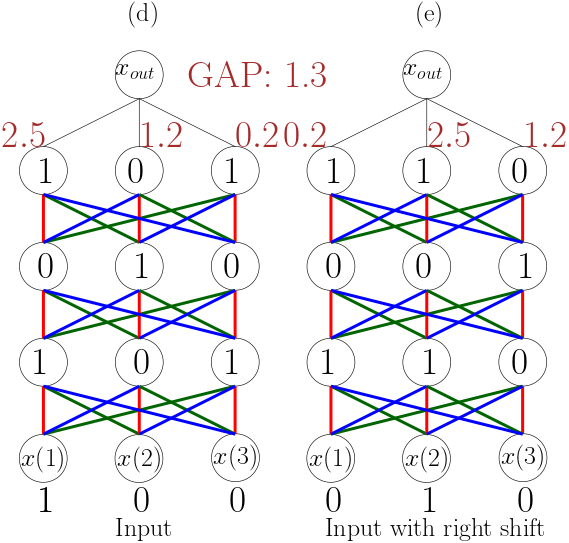
\includegraphics[scale=0.5]{figs/nnconv.png}
%}
%\end{minipage}
\caption{Illustration of the `path-view'.}
\label{fig:cartoon}
\end{figure}

\subsection{Active Gates and Capacity}
For each input example, a set of gates are \emph{on} in each layer, and this gives rise to the sub-network of active paths for that input. This active sub-network can be said to hold the memory for a given input (see cartoon $(b)$ in \Cref{fig:cartoon}), i.e., only those active paths that pass through the active gates contribute to the output. 

We note that, for DNNs with ReLU, with no bias parameters, a dataset with $n=2$ points namely $(x,1)$ and $(x/2,-1)$ for some $x\in \R^{d_{in}}$ cannot be memorised. The reason is that the gating values are the same for both $x$ and $x/2$ (for that matter any positive scaling of $x$), and hence $\phi_{x/2,\Theta}= \phi_{x,\Theta}/2$, and thus it not possible to fit arbitrary values for $\hat{y}_t(x/2)$ and $\hat{y}_t(x)$, since $\hat{y}_t(x/2)= \hat{y}_t(x)/2$. Cartoons $(a)$ and $(b)$ in \Cref{fig:cartoon} illustrate this scale invariance for inputs $x=(1,-1,2)\in\R^3$ and $x/2=(0.5,-0.5,1)\in\R^3$:  when compared to $(a)$, pre-activation values and output of $(b)$ are scaled down by a factor $2$, and the gating values of $(a)$ and $(b)$ are identical. \cite{ben} showed that DNNs can fit even random labels, and random pixels of standard datasets such as MNIST. However, it is clear from the above illustration that for any two inputs if their active sub-networks are similar, then their outputs cannot be arbitrarily different. 

Consider the deep linear network (DNLN), wherein, the activation is an identity function, which in turn can be thought of as a network whose gates are always on. Thus, all the paths are on for all the inputs, and the DLN can be reduced to a simple matrix. On the contrary, in a DNN with ReLU activations, different inputs will fire different sub-networks thereby increasing the capacity of such networks over DLNs.

\subsection{Sensitive Gates and Soft-ReLU} 
Consider the case of gates whose pre-activation inputs are near $0$, i.e., $\pm\epsilon$. Such gates are called sensitive gates, and during training, such gates can flip from $0$ to $1$ or vice-versa. Thus, by tuning such sensitive gates, gradient descent learns the right active sub-network for each input in the dataset. Note that, in the case of ReLU, the derivative of the gate is almost surely $0$, and hence it is not possible to capture the role of sensitive gates. We call this the ReLU artefact, which we remedy by considering a soft-ReLU activation, whose gating is given by $\gamma_{sr}(q)=\frac{1}{\left(1+\exp(-\beta \cdot q)\right)}, \beta>0$, and the activation is given by $\chi_{sr}(q)=q\cdot \gamma_{sr}(q)$. In the case of soft-ReLU, the derivative of the gating with respect to the pre-activation is given by $\partial_{q}\gamma_{sr}(q)=\frac{\beta}{\left(1+\exp(\beta\cdot q)\right)\left(1+\exp(-\beta\cdot q)\right)}$ (see rightmost plot in \Cref{fig:cartoon}).
